% =========================================================
% kyber-components.tex
% =========================================================
% A breakdown of the Kyber algorithm into key components/
% kernels with explanations of each

\subsection*{Components of the Kyber Algorithm}

We have identified the following key components of the kyber algorithm through profiling. 
These components are essential to the algorithm and are the focus of our optimization efforts as 
they dominate the runtime of the algorithm.
\begin{itemize}
    \item Random/Noise Sampling (25\%)
    \item Number Theoretic Transform (NTT) and Inverse NTT (30\%)
    \item Montgomery Reduction (35\%)
\end{itemize}

\begin{figure}
    \centering
    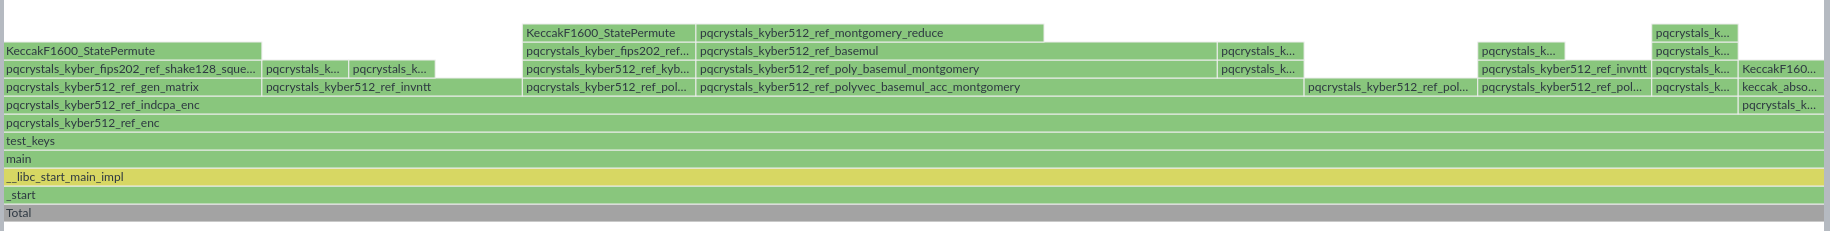
\includegraphics[width=\linewidth]{imgs/flame-graph.png}
    \caption{Flame graph of the reference software Kyber implementation}
    \label{fig:intro-timeline}
\end{figure}

\paragraph{Random/Noise Sampling.}
Random seeding, generated from expanding a uniformly random matrix, is used during the key generation and encapsulation 
routine. Randomness is essential to not just the Kyber algorithm, but to many modern cryptographic algorithms as it
and avoid determinism in generated keys and ciphertexts, and protects the algorithm against direct/side-channel attacks 
that exploit predicatability in the system. Noise sampling, on the other hand, is critical to the hardness of solving 
the learning-with-errors problem, which is the basis of the Kyber algorithm. NTT uses centered binomial noises problem.
It is important to note that a deterministic noise generator would compromise the security of the algorithm as it reduces
the LWE problem to the weaker learning-with-rounding(LWR) problem.

\paragraph{Number Theoretic Transform} is a generalization of the Discrete Fourier Transform (DFT) that has become 
increasingly important in Post Quantum Cryptography algorithm. It is fast (with a computational complexity of 
$O(n\log n)$), memory conserving, and can be implemented in a small code space. 
Almost all lattice-based crytopgraphy algorithms have been designed with parameters that support this 
fast multiplication. 
It plays an important role in Kyber as it is used to convert the polynomial multiplication in the polynomial ring to 
a multiplication in the number theoretic ring. 

\paragraph{Montgomery Reduction} is a technique for performing fast modular multiplications. By converting two numbers
$a$ and $b$ into Montgomery form, the algorithm can compute $ab \text{ mod } N$ efficiently, avoiding expensive division
operations. It is used in many important cryptographic algorithms, including RSA aand Diffie-Hellman key exchange. 
It is slower than a conventional Barret reduction for single products but is significantly faster for many 
modular multiplications in a row. In Kyber, both Montgomery and Barret reduction are used to reduce the runtime of the
algorithm.